\problemname{Circular Painting}

\illustration{0.4}{sign}{The sign outside the university.}%
It has been decided that the sign outside the university is too small, and a
new and much bigger sign should be constructed. A huge wooden panel of
sufficiently large dimensions has been built, and now you've been tasked with
painting the university's logo on this panel.

The logo is composed of disjoint circular sectors around a complete circle, and
you've been given instructions for how to paint the logo in terms of these
sectors. Starting from a horizontal angle to the right, and proceeding in
counterclockwise direction, each part of the logo is painted as a circular
sector of a given angle, inner radius, and outer radius.

\begin{figure}[h!]
  \centering
  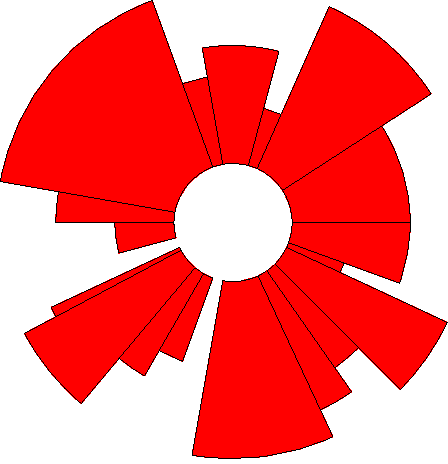
\includegraphics[width=0.30\textwidth]{logo}
  \caption{Illustration of Sample Input 3.}%
  \label{fig:sample3}
\end{figure}

The only thing you're missing is the paint. In order to estimate the amount of
paint needed, you decide to calculate the total area that the circular sectors
will cover on the sign.

\section*{Input}
The input consists of:
\begin{itemize}
    \item One line with one integer $n$ ($1 \le n \le 360$), the number of circular sectors.
    \item $n$ lines, the $i$th of which contains three integers $d$, $r_1$ and $r_2$ ($1\le d\le 360$, $0 \le r_1 \le r_2 \le 1\,000$), the angle in degrees, inner radius in centimetres, and outer radius in centimetres of the $i$th circular sector. $r_1=r_2$ is used to represent an empty circular sector of the given angle.
\end{itemize}

The sum over angles of all circular sectors equals $360$.

\section*{Output}
Output the total area of the circular sectors in square centimetres.

Your answer should have an absolute or relative error of at most $10^{-3}$.

